\section{Examen 1.- Administración de fallas con mínimos cuadrados}
\subsection{Ejercicio 1: Definición de umbrales}
\noindent
Para llevar a cabo la definición de umbrales, realizamos el método propuesto por CISCO; consiste en hacer una lectura de datos por un periodo de tiempo (en este caso fueron 10 minutos), almacenar los datos obtenidos y generar una tabla de dispersión y con base en ella definir el umbral GO (umbral mayor) y a partir de este definir los umbrales inferiores. En este caso el agente que íbamos a monitorear se nos fue proporcionado por la profesora, el cual tenía los siguientes valores.
\begin{figure}[H]
  \centering
    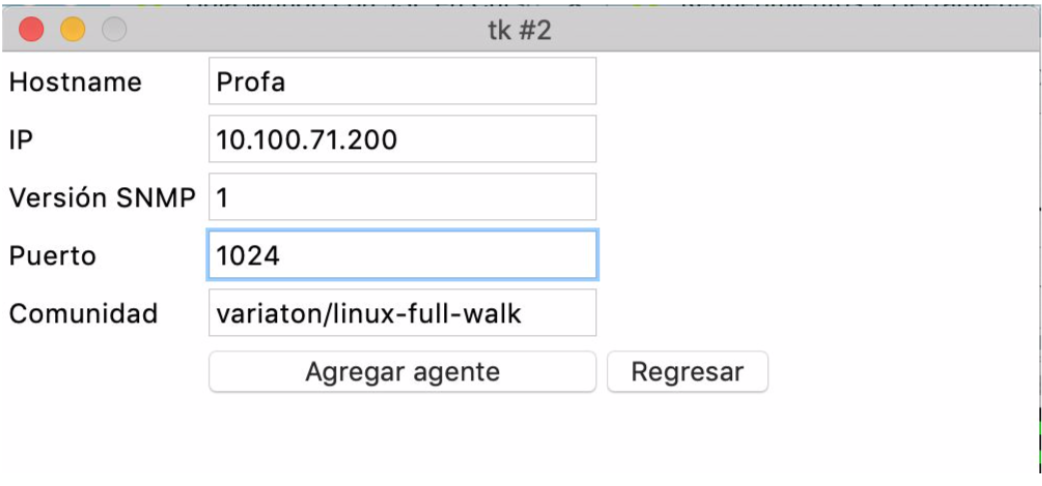
\includegraphics[scale=.8]{imagenes/primero/1-1.png}
    \caption{Agente}
\end{figure}
Una vez que fue ejecutado el programa y la lectura de los datos de uso de CPU se llevó a cabo en el plazo indicado, se obtuvo la siguiente tabla.
\begin{figure}[H]
  \centering
    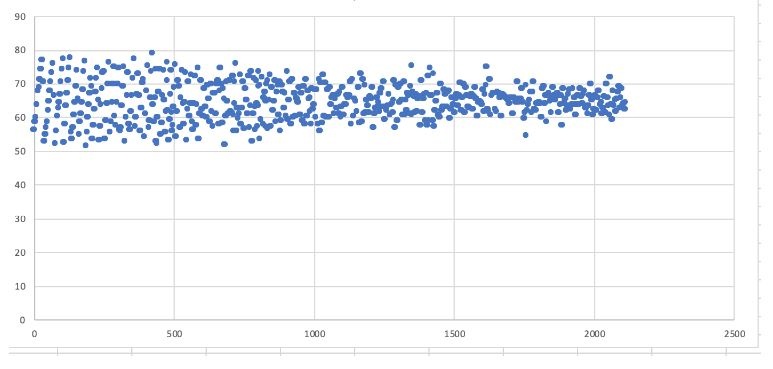
\includegraphics[scale=1]{imagenes/primero/1.JPG}
    \caption{Tabla de Dispersión}
\end{figure}
\subsection{Ejercicio 2: Mínimos Cuadrados}
\noindent
Una vez obtenidos los umbrales por medio de la tabla de dispersión se definieron dentro de nuestro sistema con el fin de poder hacer una predicción por medio del método de mínimos cuadrados, además en la gráfica se indica cuando ocurrirá un error y los colores varían cada que uno de los umbrales es rebasado; la línea de mejor ajuste se muestra de color amarillo.
\begin{figure}[H]
  \centering
    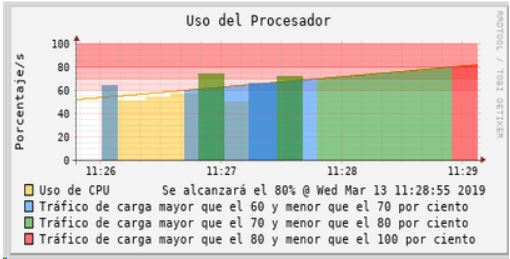
\includegraphics[scale=1.5]{imagenes/primero/2.JPG}
    \caption{Lectura del procesador}
\end{figure}
\noindent
En la gráfica se puede observar que el umbral GO es del 80\%. También, en las descripciones de la gráfica se encuentra el tiempo en el que el uso del CPU va a alcanzar ese umbral. Este tiempo es: 13 de marzo del 2019 a las 11:28:55. Para poder llevar a cabo este ejercicio se hizo uso del código siguiente.
\begin{figure}[H]
  \centering
    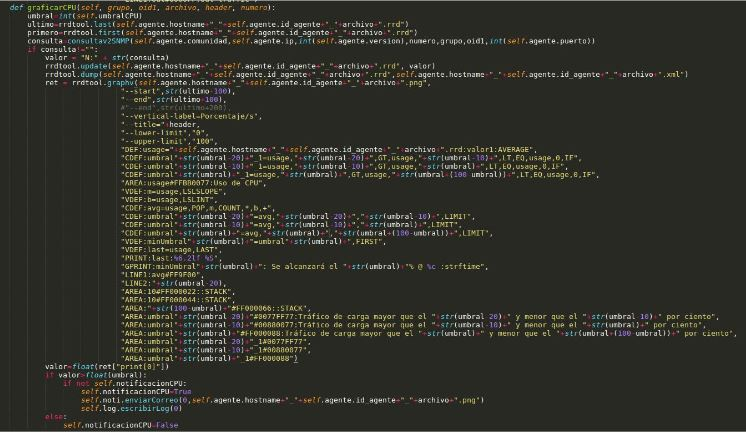
\includegraphics[scale=1]{imagenes/primero/3.JPG}
    \caption{Mínimos Cuadrados}
\end{figure}
\subsection{Ejercicio 3: Envío de Correos}
\noindent
Este ejercicio consistió en enviar un correo a la dirección de la profesora \textbf{tanibet.escom@gmail.com} en el momento en que se presentara una falla con fecha y hora del momento en el que ocurrió.
\begin{figure}[H]
  \centering
    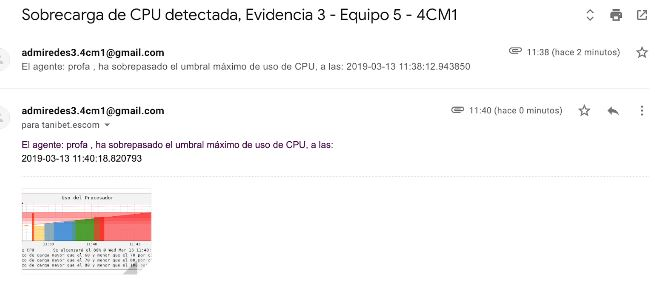
\includegraphics[scale=1.1]{imagenes/primero/4.JPG}
    \caption{Correo Enviado}
\end{figure}
\noindent
Para llevar a cabo este proceso se utilizó el siguiente código que nos permite crear el contenido de un correo y enviarlo a la dirección especificada con la información definida.
\begin{figure}[H]
  \centering
    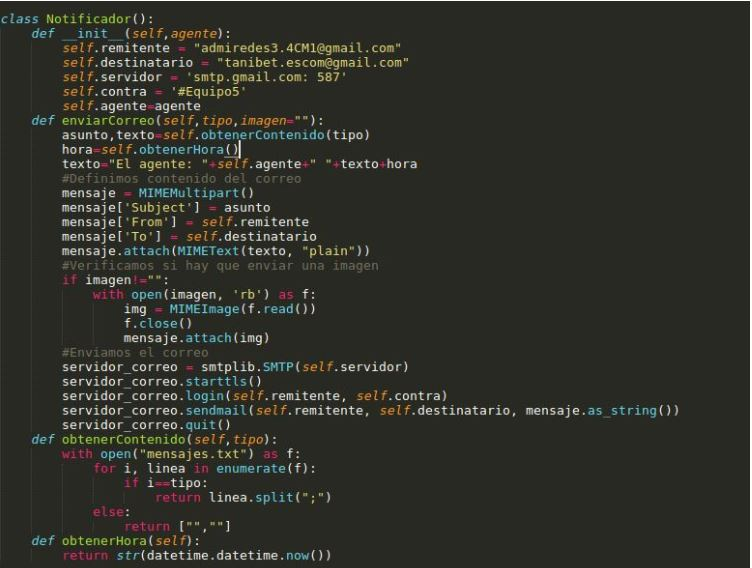
\includegraphics[scale=.8]{imagenes/primero/5.JPG}
    \caption{Envío de Correos}
\end{figure}
\subsection{Ejercicio 4: Lectura Completa}
\noindent
Para el ejercicio final, se tenia que llevar a cabo la lectura de los siguientes 3 parámetros: Uso de CPU, RAM y Disco Duro, además se tenían que mostrar las gráficas elaboradas en la práctica 1 y de igual manera, era necesario enviar el correo de notificación de que un error había ocurrido.
\begin{figure}[H]
  \centering
    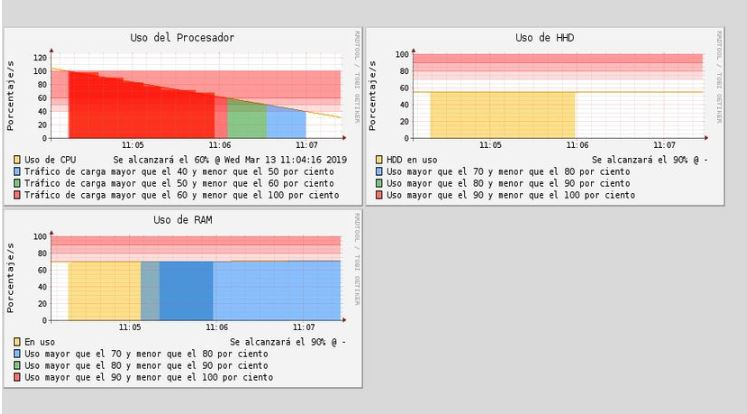
\includegraphics[scale=1]{imagenes/primero/6.JPG}
    \caption{Lectura de RAM,HDD y CPU}
\end{figure}
\begin{figure}[H]
  \centering
    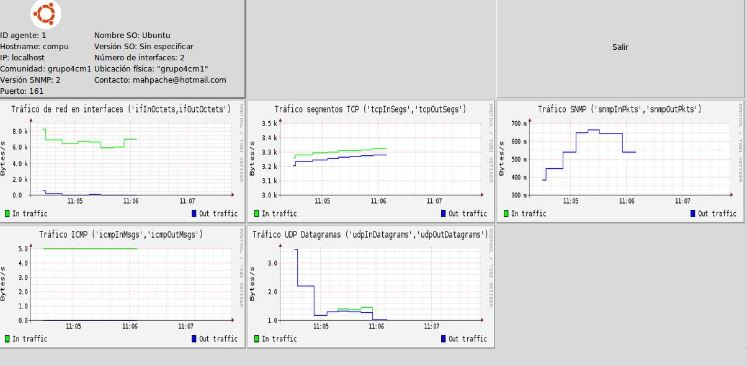
\includegraphics[scale=1]{imagenes/primero/7.JPG}
    \caption{Lectura de datos (Práctica 1)}
\end{figure}